\documentclass[11pt,a4paper,sans]{moderncv}
\usepackage[T1]{fontenc}
\usepackage[utf8]{inputenc}
\usepackage[english]{babel}
\usepackage{textcomp}

\moderncvstyle{classic}
\moderncvcolor{blue}

\usepackage[scale=0.75, top=0.5in, bottom=1in,left=0.8in,right=0.75in]{geometry}
\setlength{\hintscolumnwidth}{3.35cm}
\graphicspath{{../img/icons/}}

\nopagenumbers
\widowpenalty=0

\firstname{Andrey}
\familyname{Akinshin}

\mobile{+7-913-240-02-04}
\email{andrey.akinshin@gmail.com}
\homepage{http://aakinshin.net}{http://aakinshin.net}
\photo[70pt][0.4pt]{./photo}

%----------------------------------------------------------------------------------------

\begin{document}
	
\makecvtitle

\section{Enterprise programming}
\cvitem{}{\myemph{Microsoft .NET MVP (2015), Lead .NET Developer}}
\cvitem{Main skills}{.NET/C\#, R, Algorithms, Mathematics, Architecture design}

\cvitem{09/2010--Present}{
    
\includegraphics[height=12px]{perpetuum}
    \myhref{http://www.perpetuumsoft.com/}{{Perpetuum Software LLC}} / 
    
\includegraphics[height=12px]{enterra}
    \myhref{http://www.enterra-inc.com/}{{Enterra, Inc}} / 
    
\includegraphics[height=12px]{notariat}
    \myhref{http://notariatsoft.ru/}{{Adaptive Technologies}}
    \newline
    \phantom{~~~~}
    \mbox{
        \begin{tabular}{ll}
            09/2010--08/2011     & \myemph{Junior Software Developer}\\
            09/2011--01/2013     & \myemph{Software Developer}\\
            02/2013--Present~~~~ & \myemph{Lead Software Developer}\\
        \end{tabular}
    }
}
\cvitem{}{
    \pseudoitem
    
\includegraphics[height=12px]{pv}
    \myhref{http://passportvision.ru/}{PassportVision}:
     Software for recognizing data from document scans.\newline Team Lead, responsible for the architecture design and recognition algorithms.
}
\cvitem{}{
    \pseudoitem
    
\includegraphics[height=12px]{grapholite}
    \myhref{http://grapholite.com/}{Grapholite}: 
    Diagram editor for
    \myhref{http://apps.microsoft.com/windows/app/grapholite-diagrams-pro/99164828-b985-44ad-af71-58827d8d8a13}{
\includegraphics[height=12px]{windows8}}
    \myhref{http://www.windowsphone.com/en-us/store/app/grapholite-diagrams-phone-edition/4e89fe82-db21-45c5-a284-8de9a443fb70}{
\includegraphics[height=12px]{winphone}}
    \myhref{https://grapholite.com/Download/Grapholite.msi}{
\includegraphics[height=12px]{wpf}}
    \myhref{https://grapholite.com/Designer}{
\includegraphics[height=12px]{silverlight}}
    \myhref{https://itunes.apple.com/us/app/grapholite-diagrams-flow-charts/id954302708?ls=1&mt=8}{
\includegraphics[height=12px]{ios}}
    \myhref{https://play.google.com/store/apps/details?id=com.grapholite.diagramsdemo}{
\includegraphics[height=12px]{android}}  
    (an~analogue of MS~Visio).\newline
    Responsible for algorithms, mathematics, and architecture design. 
}
\cvitem{}{
    \pseudoitem
    
\includegraphics[height=12px]{knockout-mvc}
    \myhref{http://knockoutmvc.com/}{Knockout MVC}:~
    ASP.NET MVC wrapper for knockout.js.\newline
    Main developer: architecture design, API, main logic, official site, docs, etc. 
}
\cvitem{}{
    \pseudoitem
    
\includegraphics[height=12px]{ui-controls}
    \myhref{http://www.perpetuumsoft.com/Windows8-UI-Controls.aspx}{UI Controls for Windows 8}: 
    A set of UI controls for Windows Store apps.\newline
    Main developer: architecture design, API, XAML-layout, demo project, etc. 
}

\section{Science}
\cvitem{}{\myemph{PhD in Mathematics and Computer Science, Postdoctoral Research Fellow}}
\cvitem{08/2012--Present}{
    
\includegraphics[height=12px]{math-nsc}
	\myhref{http://www.math.nsc.ru/}{Sobolev Institute of Mathematics SB RAS} (Novosibirsk, Russia)\newline
	\myhref{http://a-server.math.nsc.ru/IM/lbrt.asp?CodLB=59}{Laboratory of Inverse Problems of Mathematical Physics}
      \newline
      \phantom{~~~~}
      \mbox{
          \begin{tabular}{ll}
              08/2012--06/2014     & \myemph{Engineer}\\
              07/2014--Present~~~~ & \myemph{Research scientist}\\
            \end{tabular}
        }
}
\cvitem{}{	
	Areas of expertise: bioinformatics, gene networks, bifurcation theory.\newline
	The grants \myhref{http://www.rfbr.ru/rffi/ru/contests_results2012/o_64737}{RFBR 12-01-00074}, RFBR 15-01-00745 A.
}
\cvitem{10/2014--Present}{
    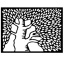
\includegraphics[height=12px]{weizmann}
	\myhref{http://www.weizmann.ac.il/}{Weizmann Institute of Science} (Rehovot, Israel)\newline \myhref{http://www.wisdom.weizmann.ac.il/}{Faculty of Mathematics and Computer Science}
     \newline
     \phantom{~~~~}
     \mbox{
         \begin{tabular}{ll}
             10/2014--Present~~~~ & \myemph{Postdoctoral Research Fellow}\\
            \end{tabular}
        }
}
\cvitem{}{
	Areas of expertise: digital signal processing, Fourier transform, Gibbs phenomenon.
}

\section{Competitive programming}
\cvitem{}{
	
\includegraphics[height=12px]{neerc}
	Final of Russian Olympiad in Informatics \myhref{http://neerc.ifmo.ru/school/archive/2005-2006/ru-olymp-roi-2006-standings.html}{ROI 2006}: \myemph{Gold medal}
}
\cvitem{}{
	
\includegraphics[height=12px]{acm-icpc}  
	\myhref{http://icpc.baylor.edu/community/results-2008}{ACM International Collegiate Programming Contest 2008}: \myemph{Certified participant}
}
\cvitem{}{
	
\includegraphics[height=12px]{acm-icpc}
	\myhref{http://icpc.baylor.edu/community/results-2009}{ACM International Collegiate Programming Contest 2009}: \myemph{Silver medal}
}


\section{Teaching}
\cvitem{09/2006--05/2012}{
	
\includegraphics[height=12px]{s42}
	\myemph{Coach} of competitive programming teams at the Barnaul \myhref{http://s42.asu.ru/}{Gymnasium №42}.
} 
\cvitem{09/2009--06/2012}{
	
\includegraphics[height=12px]{aeli}
	\myemph{Senior lecturer} of computer science at the	Altai Economics and Law Institute.
}
\cvitem{09/2009--06/2012}{
	
\includegraphics[height=12px]{ministry}
	\myemph{Lecturer}
	under the Russian federal program \myhref{http://miptic.ru/nir/podgotovka.html}{F-263 №4}.
}

\section{Selected open source projects}
\cvitem{\myhref{https://github.com/AndreyAkinshin/ProblemBook.NET}{ProblemBook.NET}}{
	Online book with compilation of .NET and C\# problems
}
\cvitem{\myhref{https://github.com/AndreyAkinshin/Russian-Phd-LaTeX-Dissertation-Template}{Phd-LaTeX-Template}}{
	\LaTeX-template for Russian Phd thesis 
}
\cvitem{\myhref{https://github.com/AndreyAkinshin/BenchmarkDotNet}{BenchmarkDotNet}}{
	.NET library for benchmarking 
}
\cvitem{\myhref{https://github.com/AndreyAkinshin/InteropDotNet}{InteropDotNet}}{
	Cross-platform AnyCPU P/Invoke for .NET 
}
\cvitem{\myhref{https://github.com/AndreyAkinshin/CultureInfoExplorer}{CultureInfoExplorer}}{
	WPF-explorer of CultureInfo instances in .NET 
}

\section{Selected public talks}
\cvitem{\myhref{http://msk2014.dotnext.ru/}{.NEXT 2014 Moscow}}{
    ``Let's talk about different .NET versions''
}
\cvitem{\myhref{http://spb2015.dotnext.ru/}{.NEXT 2015 Piter}}{
    ``Let's talk about micro-optimizations in .NET applications''
}
\cvitem{\myhref{http://dotnetconf.ru/}{.dotnetconf 10}}{
    ``Practical .NET applications optimization approaches''
}
\cvitem{\myhref{http://dotnetconf.ru/}{CLRium \#2}}{    
    ``CoreCLR, RyuJIT, and DNX''
}


\section{Selected certificates}
\cvitem{07/2014}{
	\myhref{http://aakinshin.net/data/certificates/mcp.pdf}{Microsoft Certified Professional (MCP)}
}
\cvitem{12/2014}{
	\myhref{https://www.coursera.org/account/accomplishments/specialization/44Y2uInkEe}{Data Science, a 10-course specialization by Johns Hopkins University on Coursera}
}


\section{Profiles}
\cvitem{CV and blog}{
	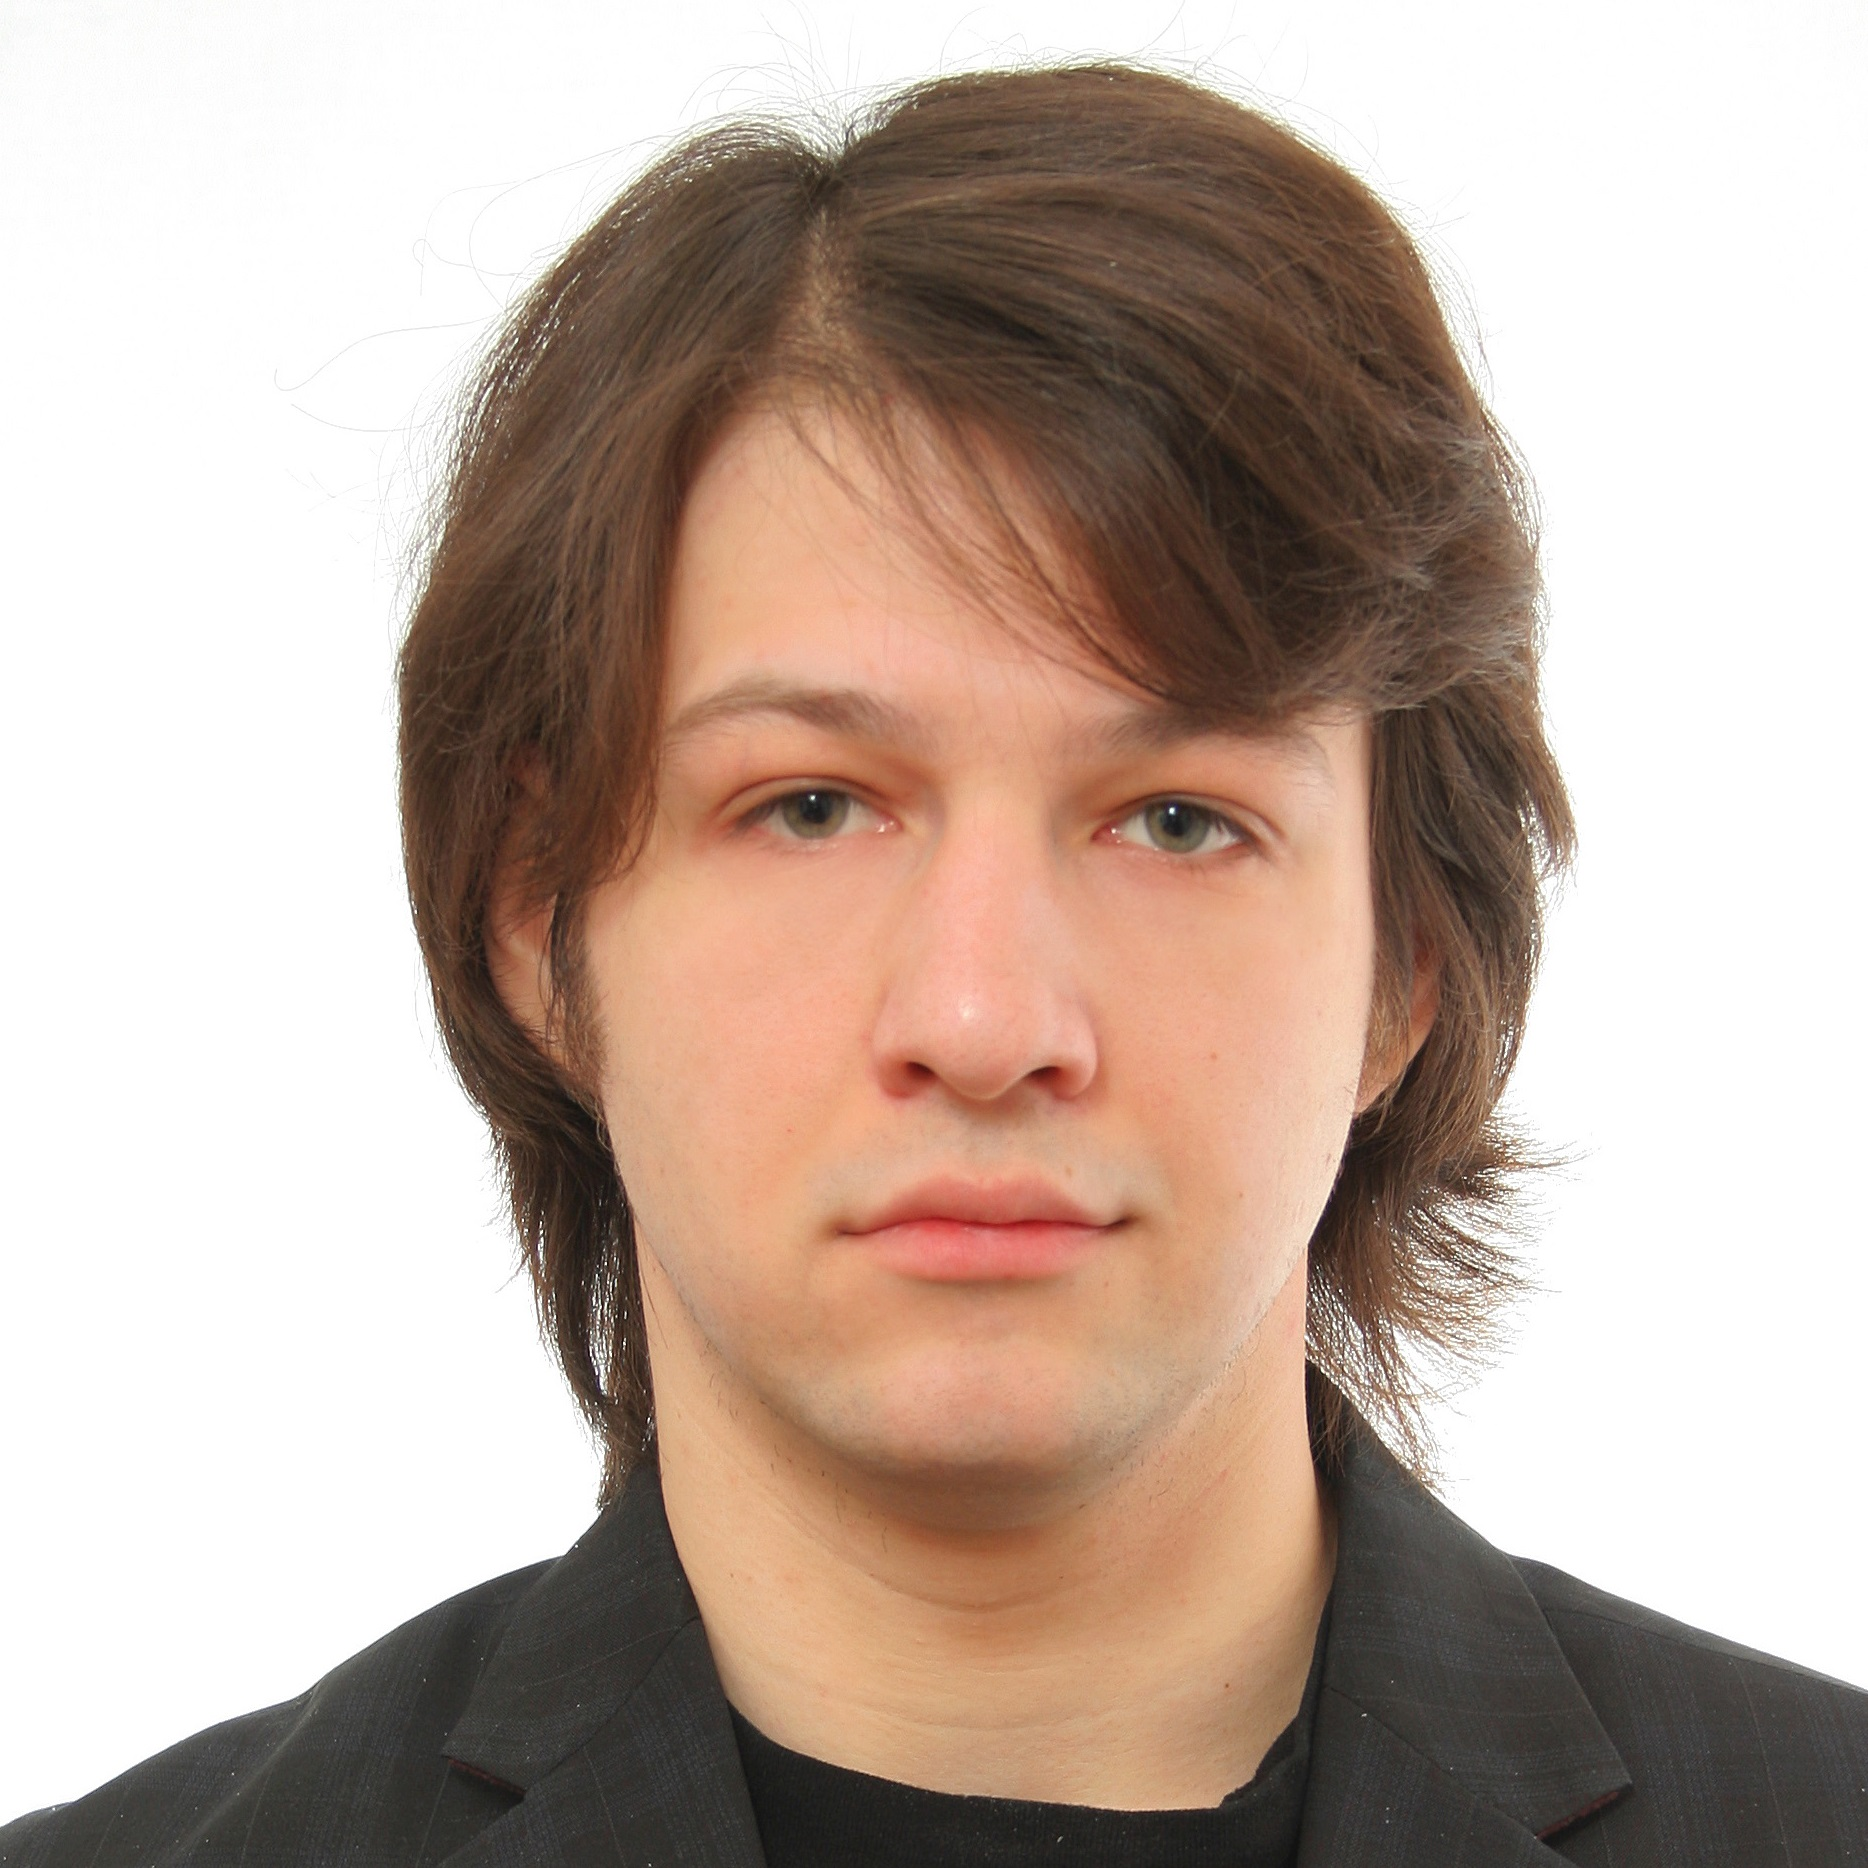
\includegraphics[height=12px]{./photo}
	\myurl{http://aakinshin.net}
}
\cvitem{GitHub}{
	
\includegraphics[height=12px]{github}
	\myurl{https://github.com/AndreyAkinshin}
}
\cvitem{StackOverflow}{
	
\includegraphics[height=12px]{stackoverflow}
	\myurl{http://stackoverflow.com/users/184842/AndreyAkinshin}
}
\cvitem{Habrahabr}{
	
\includegraphics[height=12px]{habr}
	\myurl{http://habrahabr.ru/users/dreamwalker}
}
\cvitem{LinkedIn}{
	
\includegraphics[height=12px]{linkedin}
	\myurl{http://www.linkedin.com/in/AndreyAkinshin}
}
\cvitem{SlideShare}{
    
\includegraphics[height=12px]{slideshare}
    \myurl{http://www.slideshare.net/AndreyAkinshin}
}
\cvitem{Google Scholar}{
    
\includegraphics[height=12px]{google-scholar}
    \myurl{http://scholar.google.ru/citations?user=rYVl83IAAAAJ}
}


\end{document}